%Chapter 1: Introduction

\chapter{Introduction}

The concepts of early warning and rapid response in natural hazards, particularly in seismology are multidisciplinary. They include both the societal aspects of how we respond to hazards and the physics behind these phenomena. As we seek to gain knowledge about Earth processes we must also consider the practical implications of our research. The number of people and infrastructure located in areas of earthquake and tsunami hazard is growing constantly. The problem of mitigating risk can be confronted from two perspectives. One is to minimize the hazard by moving people and infrastructure away from earthquake and tsunami-prone areas. This is unfeasible for densely populated areas (such as Japan) or already existing cities. The second approach is to minimize vulnerability by making infrastructure more resistant to the effects of natural hazards. In seismology this has lead to the creation of building codes that take into account the local hazard. This is a tricky proposition, in general the stronger a structure becomes the more expensive it is to build. Thus building codes aim to provide a balanced assessment of what can realistically be expected in terms of hazard offset by economic considerations.

Additionally, as technology and science have advanced knowledge of Earth processes it's become increasingly commonplace to provide early warnings and rapid assessments immediately following large scale disasters. In seismology many countries operate some form of earthquake early warning \citep{allen2009} system, some, such as Japan and Mexico have been operational for well over 20 years. Philosophies on how to approach this problem vary and are mostly contingent on the type of hazard the system is planned for (subduction zone vs. transform boundary events). Systems that rely on networks of stations range from those that analyze the peak displacement and frequency of the P wave \citep{kamigaichi2009} providing a faster assessment of the source but with increased uncertainty. Others use the S wave \citep{espinosa2009} which provides less uncertainty albeit with a longer waiting period. Other systems are capable of issuing warnings with a single station \citep{nakamura2007} and are typically used for stopping trains, power plants and other critical infrastructure.

Whatever strategy they employ, earthquake early warning systems really on traditional seismic sensors, seismometers and accelerometers. However, it's been observed before that these systems suffer from a condition known as saturation \citep{Brown2011} where at large magnitude it becomes increasingly difficult to separate one earthquake from another. Consider the Figure \ref{fig_pd_scaling} from \citet{Crowell2013} where a typical scaling law often used in earthquake early warning, $P_d$, the peak ground displacement of the P wave \citep{wu2007_Pd} is calculated for a range of earthquake magnitudes. The figure shows that at about M7 the peak displacement of the P wave is very similar for earthquakes between M7 and M9. There's debate in the literature as to whether this is due to the physics of the source, i.e. is rupture deterministic or not \citep{olson2005}

\begin{figure}[!ht] 
  \centering
  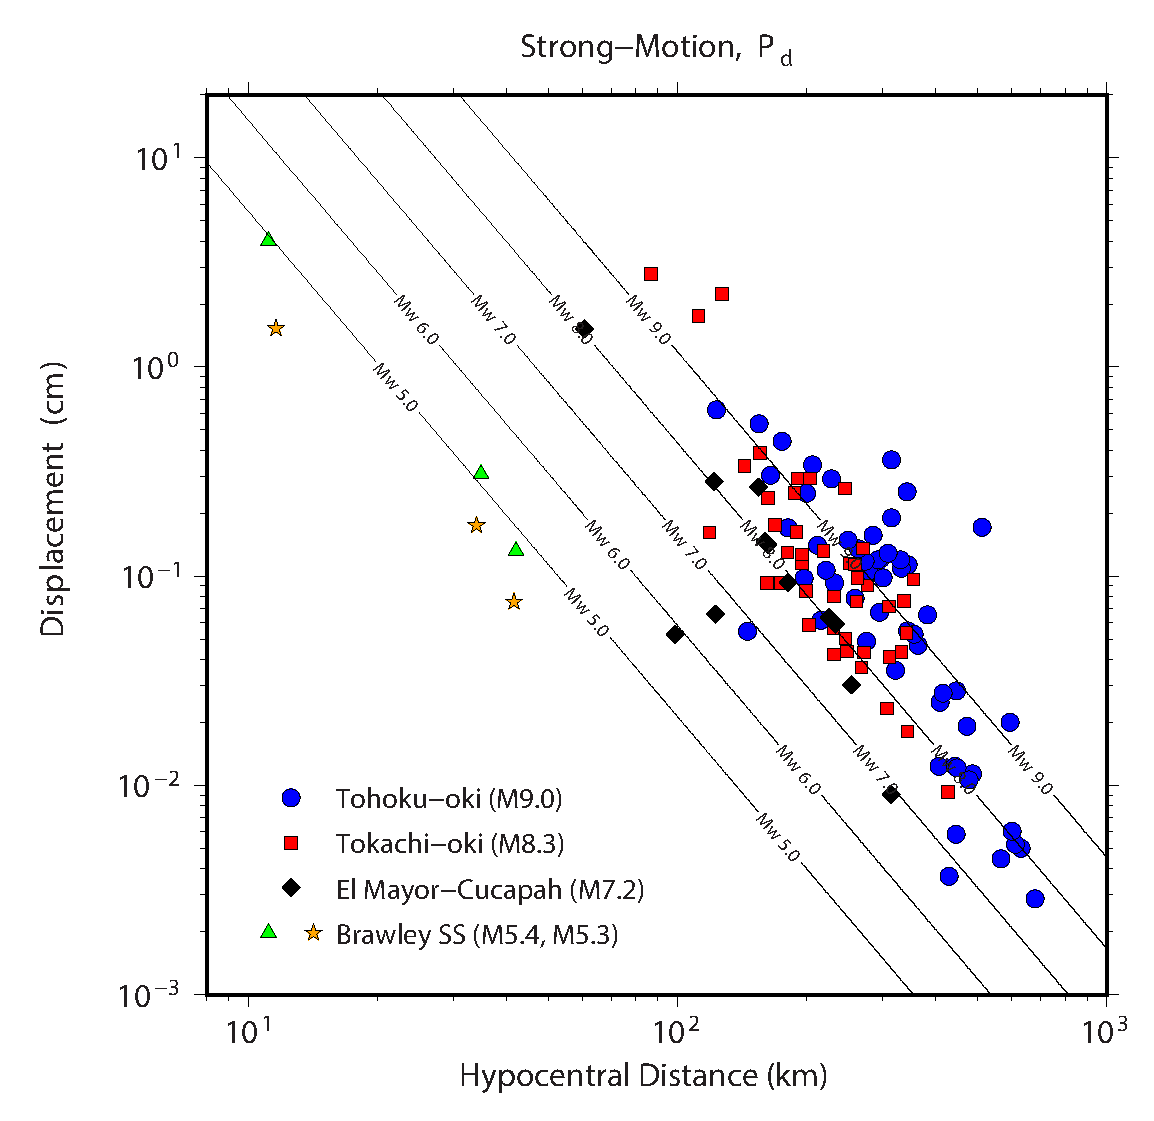
\includegraphics[width=0.99\linewidth]{./figures/ch1/pd_scaling.pdf}
    \caption[Strong motion $P_d$ scaling]{Strong motion P wave $P_d$ scaling for 5 earthquakes. The solid black lines show the regression relations for magnitude as a function of hypocentral distance. Modified from \citep{Crowell2013}}.
  \label{fig_pd_scaling}
\end{figure}

Theoretically, it's well known that as magnitude increases the spectrum of seismic radiation will become enriched in long period energy \citep{haskell1964total,brune1970} so it's tantalizing to consider that perhaps the saturation problem is instrumental rather than physical. At local distances from large earthquakes, where saturation occurs in early warning scaling laws, seismologists must rely on strong motion sensors whose low gains permit the instrument to stay on scale during shaking. These sensors, however, are affected by un-modeled rotational motions \citep{Trifunac2001} that render the long period part of the spectrum, at periods roughly longer than 10s, difficult if not impossible to use reliably \citep{Boore2005}.

In Chapter 2 we will propose and discuss at length a solution to this problem. By incorporating direct measurements of ground displacement from GPS through a real-time Kalman filter framework we will show through extensive testing during shake table tests, the M7.2 El Mayor-Cucapah and M9 Tohoku-oki earthquakes that the combination dataset, which we dub \textit{seismogeodetic} provides complete spectral recovery from 0 frequency to the accelerometer Nyquist frequency regardless of the intensity of shaking. In fact \citep{Crowell2013} used the seismogeodetic method described here to demonstrate substantial improvement in the saturation of the $P_d$ scaling law, broadband strong motion displacement and velocity waveforms are achievable through the combination of geophysical sensors.

For early warning a simple characterization of the earthquake suffices, only a rough location and estimate of magnitude or of expected shaking intensity is necessary to trigger an alert. However, immediately following rupture more elaborate models of the source are necessary to guide rapid response. For example the USGS's Shakemap \citep{allen2009shake} and PAGER \citep{jaiswal2010} data products provide a rapid assessment of expected shaking though out the epicentral area as well as of economic impacts and loss of life. The first iterations of these data products rely on simple point source models. They are often revised hours after the event when more complex source models become available. In fact, everything else being equal, considering a point source vs. a finite extent source model can have a significant impact in the Shakemap computation \citep{colombelli2013}.

In Chapter 3 we will show how both GPS and the seismogeodetic framework can be used to rapidly compute source models of increasing complexity. In particular using the permanent deformation (the static field) from an earthquake we can construct a suite of models that range from point source moment tensors to line source moment tensors and fully heterogenous slip inversions. The static field is the longest period information that is measurable from an earthquake, effectively nullifying any saturation concerns.  We will demonstrate this for the M7.2 El Mayor-Cucapah, M8.3 Tokachi-oki and M9 Tohoku-oki events. Throughout that chapter we will place particular emphasis in techniques and strategies for automation of the algorithms; removing the network operator from the computation is paramount to the success of any rapid source assessment strategy.

A more complete description of the source must include the time dependent behavior of rupture. Due to the unreliability of strong motion sensors at low frequencies automated kinematic slip inversions are only computed with tele-seismic data \citep{ji2002} and are only available hours after the event. In Chapter 4 we will demonstrate how seismogeodetic data can be used to compute kinematic models of the source. Utilizing the combination of local and regional GPS and strong motion recordings means that these models could be available within minutes of rupture initiation.

The afore mentioned models can have a significant impact in tsunami early warning as well. The tsunami warning centers (TWCs) operated by the National Oceanographic and Atmospheric Administration (NOAA) utilizing tele-seismic measurement and ocean bottom pressure measurements from DART buoys in the deep ocean. TWCs routinely provided basin scale warnings in the hours following a large event \citep{gonzalez2005,titov2005,mungov2013}. This reliance on sensors in the far field of the tsunami source means there is no warning issued to the area immediately surrounding the earthquake. Japan operates the only system designed to provide near-source warnings \citep{tatehata1997,ozaki2011}. It utilizes rapidly determined hypocenters and magnitudes from the Japanese Meteorologcal Agency (JMA) to perform a database query of precomputed scenarios. These scenarios, computed offline and well in advance of the event include intensity estimates at predetermined locations along the near-shore coast. Thus when the earthquake strikes these parameters seed the database query and the resulting model guides the warning issued to the public. During the 2011 M9 Tohoku-oki event however a strict reliance on seismic data for estimation of the earthquake source parameters lead to a severe underestimation of magnitude \citep{hoshiba2011}, once again, due to saturation. This lead to tsunamis warnings that were far too small and were not revised for many hours after the event \citep{ozaki2011}.

In Chapter 5 we will discuss the tsunami warning problem in great detail. We will propose an \textit{indirect} form of warning were the rapid models determined in Chapters 3 and 4 are used to compute the deformation of the ocean bottom, this is in turn used as the initial condition in a  fully non-linear tsunami simulation. Using the open-source code \textit{GeoClaw} \citep{leveque2011} we will produce detailed forecasts of tsunami intensity. By comparison to tsunami survey data collected immediately after the Tohoku-oki event \citep{mori2011,mori2012} we will assess the suitability of these models for forecasting. Furthermore, we will demonstrate that offshore data in the form of ocean bottom pressure and GPS buoys which directly measure the tsunami can be incorporated into a joint inverse problem. We will conclude that this joint model, which includes both land-based and ocean-based observations produces the best results and that with existing geophysical infrastructure it is reasonable to expect detailed tsunamis warnings in the shore immediately adjacent to large events.


%\appendix
%\chapter{Final notes}
%  Remove me in case of abdominal pain.

